\chapter{ATLOD: A Terrain Level of Detail (Renderer)}
This chapter describes \textit{ATLOD} (short for \textbf{A} \textbf{T}errain \textbf{L}evel \textbf{o}f \textbf{D}etail (Renderer)), the demo terrain rendering application.

\section{Preliminaries}
\subsection{Used Technologies}
ATLOD is written in C++17 and OpenGL 4.2.
For compiling build files, CMake (minimum version 3.5) is used.
ATLOD uses the following third-party libraries:
\begin{itemize}
  \item GLM: The \textit{OpenGL Mathematics (GLM)} library provides functionality for the mathematics of graphics programming, such as classes for vectors, matrices and perspective transformations.
  \item GLEW: The \textit{OpenGL Extension Wranger Library (GLEW)} is an extension loading library for OpenGL. 
  \item GLFW: \textit{GLFW} is a multi-platform library for desktop-based OpenGL applications, offering an API for managing windows, contexts and input handling.
  \item STB: STB is a collection of header-only libraries developed by Sean Barrett TODO cite. ATLOD uses \texttt{stb\_image.h} for loading images of heightmaps and textures.
\end{itemize}

The source code is hosted on GitHub on the repository AmarTabakovic/3d-terrain-with-lod
and is licensed under TODO.

\subsection{Chosen Algorithms}
The chosen algorithms and their reasons for implementing them are the following:
\paragraph{Naive Brute-force Algorithm} The naive brute-force algorithm consists of simply reading in all height values from the heightmap as vertices and rendering them directly to the screen.
The main reason for implementing the naive brute-force algorithm is to motivate the usage of terrain LOD algorithms by showing the difference in performance
compared to the optimized LOD approaches.

% TBD, depends on how far I come
\paragraph{GeoMipMapping} The main reason for implementing GeoMipMapping is to have at least one CPU-based approach
as a reference point for comparison with GPU-based approaches.
In addition, GeoMipMapping is considered to be relatively straightforward to implement \cite[p.~79]{focuson3dterrainprogramming}.

% \paragraph{Hoppe and Lossaso's Geometry Clipmaps} TODO
% \paragraph{Strugar's CDLOD} TODO

\section{Height and Texture Data}
\subsection{Data Sources}
\subsubsection{SwissTopo}

\subsubsection{SRTM}

\subsection{Supported Formats}
The following file formats are supported for loading heightmaps:
\begin{itemize}
  \item \texttt{.png} and \texttt{.jpg}: Heightmaps can be loaded as PNG and JPG images. This is implemented using \texttt{stb\_image.h}.
  \item \texttt{.asc}: Heightmaps as ASCII grids are supported. Digital elevation data from the Shuttle Radar Topography Mission (SRTM) is delivered in ASCII grid format.
  \item \texttt{.xyz}: the XYZ format is based on SwissTopo
\end{itemize}


\section{Basic Setup and Architecture}
\subsection{Overview}
TODO High-level class diagram
\subsection{Shaders}

\subsection{Camera}

\subsection{Heightmap}

\subsection{Terrain}
Each terrain LOD algorithm is encapsulated in a class, which inherits from the base terrain class \texttt{Terrain}.
The base terrain is structured as shown in listing TODO.

\section{Naive Brute-force Algorithm}
The naive brute-force algorithm, which simply renders every vertex without any LOD considerations, is encapsulated in the class \texttt{NaiveRenderer}.

The method \texttt{loadBuffers()} loads the height data from the heightmap directly into a vertex buffer with the ID \texttt{terrainVBO} and the indices into an index (i.e. element) buffer named \texttt{terrainEBO}.
The indices are organized such that they can be rendered as triangle strips with \texttt{GL\_TRIANGLE\_STRIPS}.
Each row is separated using a special marker index named \texttt{RESTART}, which is set to the maximum possible \texttt{GLuint} value and is used for the \texttt{GL\_PRIMITIVE\_RESTART} mode,
allowing for the entire terrain to be rendered in a single \texttt{glDrawElements()} call. This draw call happens every frame in the 
method \texttt{render()}. Figure~\ref{fig:naive-triangles} shows the organization of indices for rendering the terrain as triangle strips.

\begin{figure}[H]
  \centering
  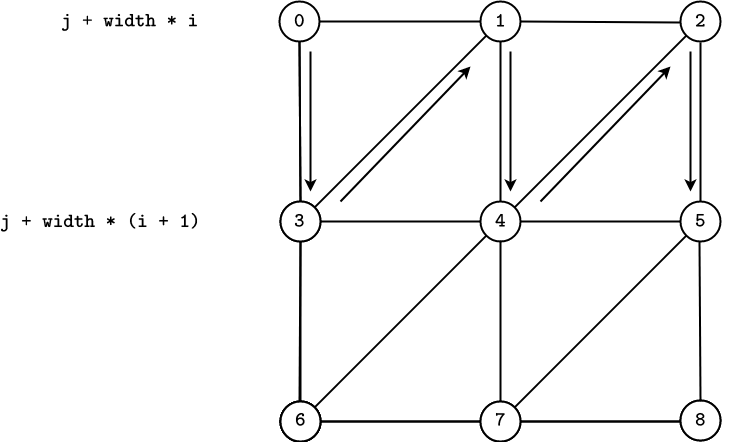
\includegraphics[width=0.9\textwidth]{naive-triangles}
  \caption{Example of a terrain layout for triangle strips. The looping index \texttt{i} goes from 0 to the terrain height and \texttt{j} from 0 to the terrain width. The final indices to be rendered are \texttt{0,3,1,4,2,5,RESTART,3,6,4,7,5,8,RESTART}.}\label{fig:naive-triangles}
\end{figure}

\section{GeoMipMapping}
ATLOD's GeoMipMapping implementation is encapsulated in the class \texttt{GeoMipMapping} and differs a bit from the 
original paper. Instead of drawing vertices directly in immediate mode and by loading each vertex manually with \texttt{glVertex},
this implementation uses vertex buffers and index buffers for rendering. 

\subsection{Data Structures}

\subsection{Vertex and Index Organisation}
Vertices are loaded into the vertex buffer in the method \texttt{loadBuffers()}. 

\subsection{Avoiding Pops}
\begin{figure}[H]
  \centering
  \subfloat[\centering \texttt{0000}.]{{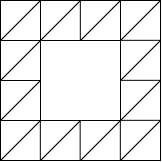
\includegraphics[width=0.17\textwidth]{atlod-geomipmapping-0000.png} }}
  \qquad
  \subfloat[\centering \texttt{0001}.]{{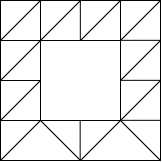
\includegraphics[width=0.17\textwidth]{atlod-geomipmapping-0001.png} }}
  \qquad
  \subfloat[\centering \texttt{0010}.]{{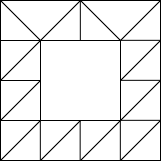
\includegraphics[width=0.17\textwidth]{atlod-geomipmapping-0010.png} }}
  \qquad
  \subfloat[\centering \texttt{0011}.]{{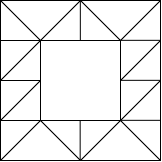
\includegraphics[width=0.17\textwidth]{atlod-geomipmapping-0011.png} }}

  \subfloat[\centering \texttt{0100}.]{{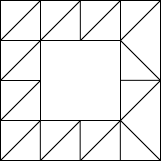
\includegraphics[width=0.17\textwidth]{atlod-geomipmapping-0100.png} }}
  \qquad
  \subfloat[\centering \texttt{0101}.]{{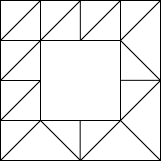
\includegraphics[width=0.17\textwidth]{atlod-geomipmapping-0101.png} }}
  \qquad
  \subfloat[\centering \texttt{0110}.]{{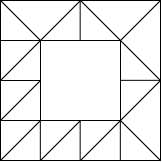
\includegraphics[width=0.17\textwidth]{atlod-geomipmapping-0110.png} }}
  \qquad
  \subfloat[\centering \texttt{0111}.]{{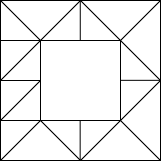
\includegraphics[width=0.17\textwidth]{atlod-geomipmapping-0111.png} }}

  \subfloat[\centering \texttt{1000}.]{{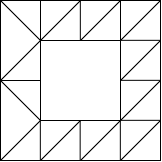
\includegraphics[width=0.17\textwidth]{atlod-geomipmapping-1000.png} }}
  \qquad
  \subfloat[\centering \texttt{1001}.]{{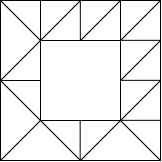
\includegraphics[width=0.17\textwidth]{atlod-geomipmapping-1001.png} }}
  \qquad
  \subfloat[\centering \texttt{1010}.]{{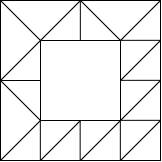
\includegraphics[width=0.17\textwidth]{atlod-geomipmapping-1010.png} }}
  \qquad
  \subfloat[\centering \texttt{1011}.]{{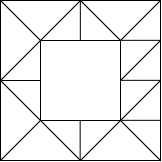
\includegraphics[width=0.17\textwidth]{atlod-geomipmapping-1011.png} }}

  \subfloat[\centering \texttt{1100}.]{{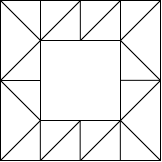
\includegraphics[width=0.17\textwidth]{atlod-geomipmapping-1100.png} }}
  \qquad
  \subfloat[\centering \texttt{1101}.]{{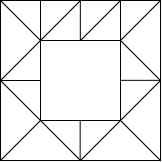
\includegraphics[width=0.17\textwidth]{atlod-geomipmapping-1101.png} }}
  \qquad
  \subfloat[\centering \texttt{1110}.]{{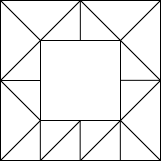
\includegraphics[width=0.17\textwidth]{atlod-geomipmapping-1110.png} }}
  \qquad
  \subfloat[\centering \texttt{1111}.]{{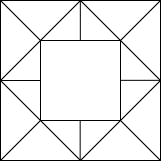
\includegraphics[width=0.17\textwidth]{atlod-geomipmapping-1111.png} }}
  \caption{Every possible border subblock configuration for a LOD 2 GeoMipMap of a $5 \times 5$ block. The bits (read from left to right) represent the left, right, top and bottom borders and are set to 1 if the bordering block on the corresponding side has a lower LOD, and 0 otherwise. The center subblocks have been omitted from the illustration.}\label{fig:atlod-geomipmapping-popping-avoidance}
\end{figure}

